\documentclass[a4paper,
DIV=13,
12pt,
BCOR=10mm,
department=FakEI,
%lucida,
%KeepRoman,
%twoside,
parskip=half,
automark,
%headsepline,
]{article}

\usepackage[utf8]{inputenc}
\usepackage{tabularx}
%\usepackage[english]{babel}
\usepackage[ngerman]{babel}
\setlength{\parindent}{0pt}
\date{\today}
\usepackage[table]{xcolor}
\usepackage{graphicx}
\usepackage{abstract}



\title{Stimmungsampel}

\author{Luzia Pfeilschifter und Felix Maier}



%\studentid{123456789 und 3124819}
%\department{Elektro- und Informationstechnik}
%\studyprogramme{Bachelor Elektro- und Informationstechnik}
%\startingdate{1.\,November 2088}
%\closingdate{11.\,Dezember 2089}			%%muss noch geändert werden

%\firstadvisor{Prof. Dr. Paula Streng}
%\secondadvisor{Prof. Dr. Petra Hart}
%\externaladvisor{Dr. Klara Endlos}

%\externallogo[height=1.5cm]{firmenlogo}

\begin{document}
\maketitle
\cleardoublepage
\begin{abstract}
Das Ziel des Projektes war es ein minimalistisches Gerät mit dem STM32G031-Microcontroller zu entwickeln, welches die Stimmung des Trägers mithilfe von LED's darstellt und dabei party-tauglich ist. Aus diesem Vorgaben ist das entwickelte Gerät entstanden. Es wird mit einer Knopfzelle betrieben und lässt sich durch eine Berührung mit dem Finger an die Vorderseite des Gehäuses zyklisch, wie eine normale Ampel, weiterschalten, dies wird durch einen kapazitiven Sensor ermöglicht. Außerdem ist noch ein Schalter verbaut, der die "Stimmung" einrasten lässt um beispielsweise ein versehentliches Weiterschalten beim Tanzen zu verhindern. Zudem ermöglicht der Schalter eine Reduktion des Stromverbrauchs, wodurch der Partyspaß noch länger anhält.
\end{abstract}
\cleardoublepage
\tableofcontents

\cleardoublepage
\section{Funktionsweise}
\begin{figure}[!hbpt]
 \begin{center} 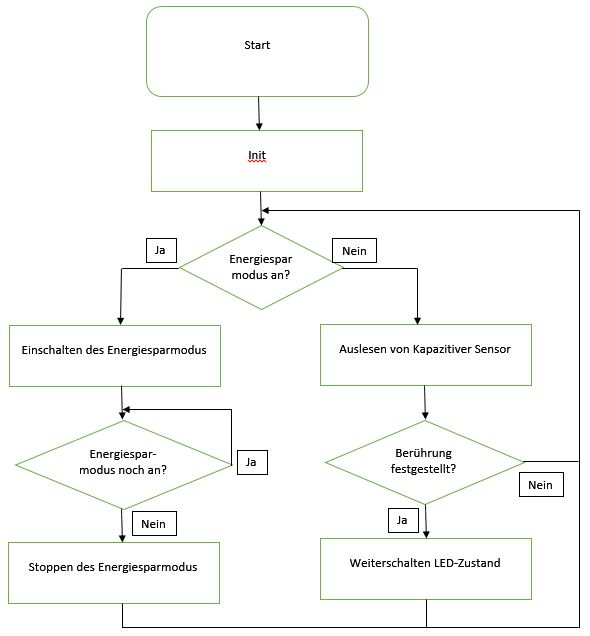
\includegraphics[width=1.2\textwidth]{AblaufMain.jpg}
 \caption{Flussdiagramm zum Ablauf des Hauptprogramms}
 \label{fig:Register}
  \end{center}
\end{figure}

\begin{figure}[!hbpt]
 \begin{center} 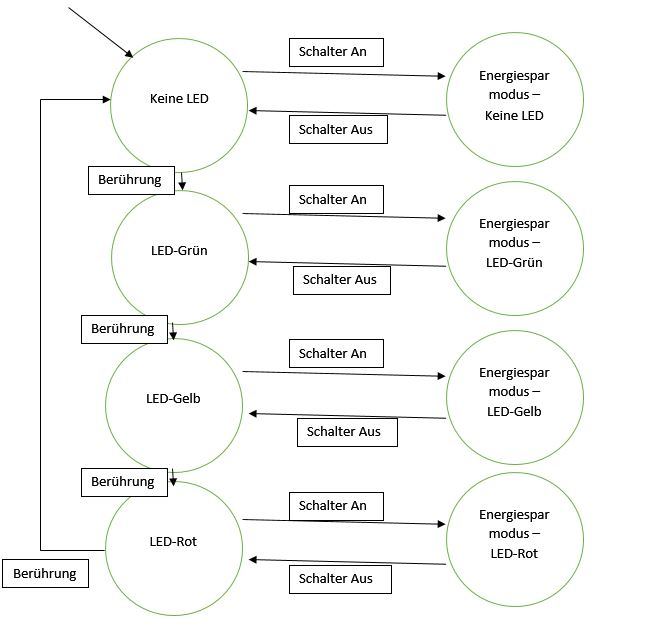
\includegraphics[width=1.2\textwidth]{Zustandsdiagramm.jpg}
 \caption{Zustandsdiagramm}
 \label{fig:Register}
  \end{center}
\end{figure}



\newpage
\section{Microcontroller}

Das Projekt wurde mit dem STM32G031J6M6 umgesetzt. Dies ist ein 8-Pin Microcontroller mit einer ARM 32-Bit Cortex–M0+ CPU, der sehr wenig Strom verbraucht und damit perfekt für diesen Einsatzbereich ist. Er kann mit 1,7V bis 3,6V betreiben werden, was gut für den Betrieb mit eine Knopfzelle ist. Zudem verfügt er über 4 Oszillatoren, einen DMA-controller, einen ADC, 11 Timer und verschiedene Kommunikationsinterfaces, was völlig ausreichend für dieses Projekt ist. Dieser Mikrocontroller hat aber auch Nachteile: Einerseits die Pin-Knappheit, da nur 6 Pins programmiert werden können, was die Komplexität der Außenbeschaltungen einschränkt. Andererseits kann es schwer sein diesen Microcontroller zu debuggen bzw. zu flashen, da die Pins 7 und 8 umprogrammiert werden können und somit nicht mehr für der Debug- bzw. Flashvorgang zur Verfügung stehen. Dieses Problem wurde mithilfe des Programmes STM32 ST-LINK Utility, welches eine "Connect under Reset"-Option besitzt, gelöst. Dabei wird der Controller in den Reset-Zustand gebraucht. Beim Austreten aus diesen Zustand wird sich mit dem Mikrocontroller verbunden bevor der bereits bestehende Code ausgeführt wird, was es erlaubt den Baustein neu zu programmieren.

\begin{figure}[!hbpt]
 \begin{center} 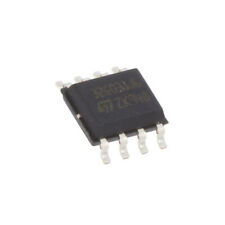
\includegraphics[width=0.8\textwidth]{s-l225.jpg}
 \caption{STM32G031J6M6 als SMD-Baustein}
 \label{fig:SMD-Baustein}
  \end{center}
   \begin{center} 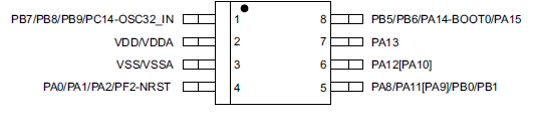
\includegraphics[width=1\textwidth]{Stm32g031j6m6.png}
 \caption{Pinbelegung des Mikrocontrollers STM32G031J6M6}
 \label{fig:SMD-Baustein}
  \end{center}  
\end{figure}
\newpage
\section{LED}
\subsection{WS2812b}
Als nächstes wird die Möglichkeit eine WS2812b-LED zu verwenden betrachtet. Sie hat von allen bisherigen LED's die größte Variation an Farben, die dargestellt werden können. Die Ansteuerung erfolgt außerdem nur über eine Datenverbindung, was bei einem Mikrocontroller mit nur 8 Pins sehr vorteilhaft ist. Die verschiedenen Übertragungsbit können dabei als PWM-Signale mit unterschiedlichen Duty-Cycle aufgefasst werden. So hat eine logische \"0\" ein Duty-Cycle von 32 Prozent und eine logische \"1\" ein Duty-Cycle von 68 Prozent. Daraus können GRB-Werte gebildet werden, welche durch ein Duty\-Cycle von 0\% über mindestens 50 $\mu$s von den LED's übernommen werden. Dieser komplette Vorgang ist sehr aufwändig für den Prozessor. Deshalb wird der im Mikrocontroller eingebaute Prozessor DMA-Controller, was für \"Direct Memory Access\" steht, verwendet, um die Auslastung des Prozessors signifikant zu verbessern. Die WS2812b LED hat aber insgesamt zwei große Nachteile, die sie schlechter als andere Varianten macht. Zum einen der hohe Preis, was mit dem Ziel einen möglichst preiswerten Aufbau zu entwerfen kollidiert. Und zum anderen die benötigt Stromversorgung von 5V, was einen Hochsetzsteller erfordern würde, da der komplette Aufbau mit einer Knopfzelle betrieben wird.

\newpage

\subsection{LED-Schaltung}
\begin{figure}[!hbpt]
 \begin{center} 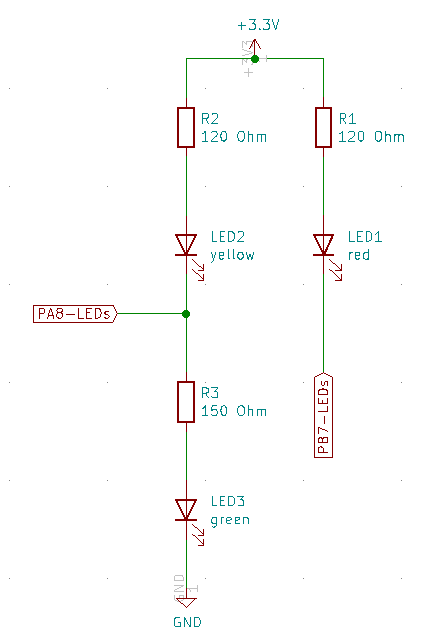
\includegraphics[width=0.8\textwidth]{LED_Schaltung.png}
 \caption{LED Schaltung}
 \label{fig:Register}
  \end{center}
\end{figure}

\newpage

Letztendlich war am interessantesten eine Schaltung, die mit möglichst wenig Pins möglichst viele LED's ansteuert. Um dies zu ermöglichen wurde eine Schaltung entworfen, die mit Hilfe von Input und Output dies ermöglicht. Dabei können bis zu 4 LED's mit 2 Pins angesteuert werden. In der vorliegenden Ampelschaltung sind nur 3 LED's notwendig, allerdings könnte die 4. noch zwischen Ground und LED1 gehängt werden, wie parallel dazu LED3. Also gibt es 3 verschiedene Zustände, die im folgenden erklärt werden:
\subsubsection{LED1 leuchtet}
Der Pin "PB7-LEDs" wird als Output auf "LOW" gesetzt. Dadurch fließt ein Strom zwischen 3.3V und dem Output "LOW" $\rightarrow$ LED1 leuchtet Damit die anderen LEDs nicht leuchten, wird "PA8-LEDs" auf Input gesetzt, dadurch wird er hochohmig und im linken Zweig fließt kein Strom.
\subsubsection{LED2 leuchtet}
Der Pin "PA8-LEDs" wird als Output auf "LOW" gesetzt. Dadurch fließt ein Strom zwischen 3.3V und dem Output "LOW" $\rightarrow$ LED2 leuchtet Damit die anderen LEDs nicht leuchten, wird "PB7-LEDs" auf Input gesetzt, dadurch wird er hochohmig und im rechten Zweig fließt kein Strom.
\subsubsection{LED3 leuchtet}
Der Pin "PA8-LEDs" wird als Output auf "HIGH" gesetzt. Dadurch fließt ein Strom zwischen dem Output "HIGH" und dem Ground $\rightarrow$ LED3 leuchtet Damit die anderen LEDs nicht leuchten, wird "PB7-LEDs" auf Input gesetzt, dadurch wird er hochohmig und im rechten Zweig fließt kein Strom.

\subsubsection{keine LED leuchtet}
Der Pin "PA8-LEDs" wird als Input deklariert, dadurch fließt im linken Zweig kein Strom. Wenn nun auch noch "PB7-LEDs" auf Input gesetzt wird, wird auch dieser Pin hochohmig und im rechten Zweig fließt kein Strom. Dadurch dass weder im linken noch im rechten Zweig ein Stromfluss entsteht sind alle LED aus, was dem letzten Zustand im Zyklus entspricht, bevor es wieder von vorne los geht mit der roten LED1.

\begin{center}
\rowcolors{3}{lightgray}{white}
\begin{tabularx}{\columnwidth}{XXXl}
Leuchtet &Zustand &PA8-LEDs &PB7-LEDs \\ \hline
LED1 & grün & IN &OUT-LOW\\
LED2 & gelb & OUT$-$LOW &IN\\
LED3 & rot & OUT$-$HIGH & IN\\
keine LED & aus & IN & IN
 
\label{tab:ZusammenfassungderFunktionsweisederLEDSchaltung}
\end{tabularx}
\end{center}

\subsection{Auswahl der Widerstände für die LED-Schaltung}

\begin{figure}[!hbpt]
 \begin{center} 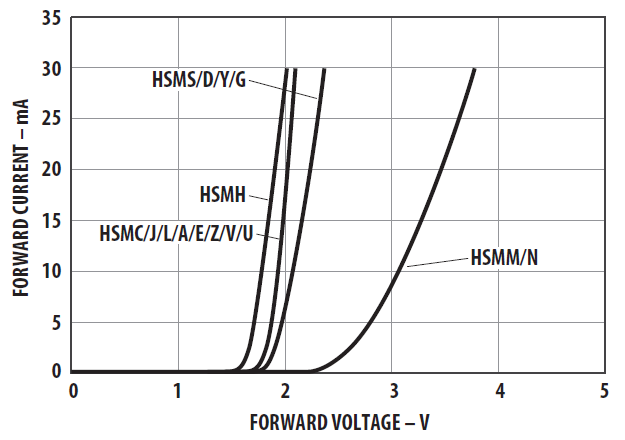
\includegraphics[width=0.8\textwidth]{Kennlinien_LED_SMD.png}
 \caption{Kennlinien forward current vs. forward voltage der unterschiedlichen SMD-LED's }
 \label{fig:Register}
  \end{center}
\end{figure}
Anhand dem Bestand im Labor der OTH, fiel die Entscheidung für die Widerstandsreihe R0603. Auch die Auswahl der LED's erfolgte nach diesem Kriterium für die HSMx-A100-Reihe von Avago. 

Hierbei ergeben sich aus dem Datenblatt unterschiedliche forward voltage für die jeweilige Leuchtfarbe. Die Berechnung der Widerstände erfolge allerdings immer nach demselben Prinzip. 
Dabei wurde zunächst die jeweilige forward voltage ermittelt und anschließend mit der Batterieversorgung von 3.3V und einem gewünschten Strom von 10mA der resultierende Widerstand berechnet. Die Festlegung auf 10mA erfolgte vor allem aus Erfahrung und aus Gründen des Stromverbrauchs. Der normale Betrieb liegt bei 20mA, dies ist allerdings recht hell und bei einer meist dunklen Party erschienen somit auch 10mA ausreichend, was günstiger für den Stromverbrauch ist.\\

Bei der roten LED1 handelt es sich um HSMS-A100-J00J1. Mit dieser Information lässt sich die entsprechende Kennlinie und damit die resultierende forward voltage von 2.1V ermitteln.
Die folgende Berechnung für den Vorwiderstand ist also:

$$ R1 = (3.3 - 2.1)V / 10mA = 120 \Omega$$

Als letztes muss noch überprüft werden, ob dieser Wert auch innerhalb der R0603-Reihe vorhanden ist oder ob ein naheliegender Wert gewählt werden muss. Da allerdings 120 $\Omega$ vorkommen, kann der exakte Wert für die Schaltung verwendet werden. \\

Die selben Schritte erfolgen nun auch für die weiteren LED's, wodurch sich für die gelbe LED2 (HSMY-A100-J00J1) dieselbe forward voltage ergibt. Dadurch ist nun die Berechnung gleich der Rechnung für die rote LED:

$$ R2 = (3.3 - 2.1)V / 10mA = 120 \Omega$$

Und auch hier kann direkt der richtige Wert aus der Reihe genommen werden.\\ 

Nun noch zur grünen LED3, dem Bauteil HSME-A100-L01J1. Also lässt sich eine forward voltage von 1.8V aus dem Diagramm ablesen. 
Dadurch ergibt sich für den Widerstand:

$$ R3 = (3.3 - 1.8)V / 10mA = 150 \Omega$$

Nach der Reihe R0603 ergibt das auch einen Widerstand von 150 $\Omega$.

\newpage
\section{Kapazitiver Sensor}
Als nächstes wird der Kapazitive Sensor erläutert, der für die Weiterschaltung der LED's zuständig ist. Grundsätzlich ist zu sagen, dass alle Kapazitiven Sensor auf einem RC-Oszillator basieren. Kommt es zu einer Berührung oder Näherung durch zum Beispiel einem Finger so wird die Kapazität und somit Lade- und Entladezeit des Oszillators erhöht. Es gibt verschieden Möglichkeiten dies zu detektieren. Nachfolgend sind einige davon aufgelistet, die für das Projekt in Betracht gezogen wurden.
\subsection{Verschiedene Varianten von Kapazitiven Sensoren}
\label{VerschiedeneKapSenVar}
\subsubsection{Komparator}
Zuerst wird die Komparator-Methode erklärt. Hierbei wird ein Dreieck-Signal an einem RC-Ladeglied angelegt. Durch das RC-Glied wird das Signal abgerundet ähnlich wie in \ref{fig:Tiefpass} zusehen. Dieses Signal und eine feste Gleichspannung wird nun an einen Komparator angelegt. Jedes Mal wenn der Komparator umschaltet wird die vergangene Zeit gemessen. Gibt es eine Berührung so wird das Dreieck-Signal stärker abgerundet und somit verändert sich auch die Zeit die der Komparator zum Umschalten braucht. Durch dieses Prinzip können auch relativ elegant Timer und Interrupts verwendet werden. 
\begin{figure}[!hbpt]
 \begin{center} 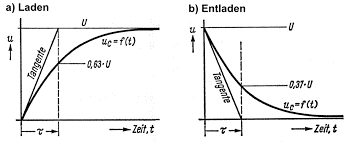
\includegraphics[width=1\textwidth]{RCTiefpass.png}
 \caption{RC-Tiefpass}
 \label{fig:Tiefpass}
  \end{center}
\end{figure}

\subsubsection{ADC}
Als nächstes wird die Variante erklärt, die einen Analog-Digital-Wandler verwendet. Hierbei wird ein RC-Ladeglied auf den logischen High-Pegel aufgeladen und nach einer festen Zeit mithilfe des ADC gemessen. Die gemessene Spannung ist dabei abhängig von der Kapazität des Ladeglieds. Ist die Kapazität nicht erhöht, also keine Berührung oder Näherung von zum Beispiel einem Finger, so entlädt sich die Spannung schneller. Gibt es aber eine Berührung oder Näherung so ist die Kapazität höher und die Entladekonstant des RC-Glieds größer, was zu einem zeitlich längeren Spannungsabfall führt. Zusammengefasst ist also die Spannung, die der ADC misst größer wenn eine Berührung oder Näherung statt gefunden hat. 
\subsubsection{Sende- und Empfangspins}
Die dritte Variante ist jeweils einen Sende- und Empfangspin zu benutzen. Dabei wird ein sehr hochohmiger Widerstand zwischen zwei Pins gesetzt, der mit der Kapazität des Receivepins ein RC-Tiefpass realisiert. Verändert man nun den Logik-Pegel am Sendpin so dauert es, wegen dem Tiefpass, eine kurze Zeit bis diese Änderung am Receivepin ankommt. Diese Zeit ist messbar und je nach Kapazität unterschiedlich. Die unterschiedliche Kapazität ist auf ein Metallstück oder Folie, welches am Receivepin befestigt ist, zurückzuführen. Berührt man diese Folie so wird, wie bei der ADC-Variante, die Ladekonstante erhöht und es dauert länger bis eine Änderung des Sendpins am Receivepin erkannt wird. Dieser Aufbau ist im Bild \ref{fig:KapSensor} veranschaulicht.

\begin{figure}[!hbpt]
 \begin{center} 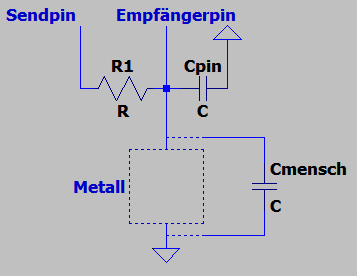
\includegraphics[width=1\textwidth]{KapazitiverSensor.png}
 \caption{Funktionsweise des Kapazitiven Sensors}
 \label{fig:KapSensor}
  \end{center}
\end{figure}

\subsection{Bewertung}
\label{Bewertung}
Als nächstes werden die Varianten aus \ref{VerschiedeneKapSenVar} bewertet. Die erste Lösung ist hier sehr umständlich umzusetzen, da der Mikrocontroller STM32G0316J6M6 keinen Komparator besitzt. Deswegen wurde diese Variante nicht verwendet. Die ADC-Methode hat den großen Vorteil, dass sie nur ein Pin benötigt. Sie bracht jedoch eine zusätzliche Kapazität, was Platz verbraucht und Kosten verursacht. Zudem besitzt der Mikrocontroller nur einen Analog-Digital-Wandler, welcher gegebenenfalls anderweitig für einen Sensor hätte verwendet werden können. Die letzte Variante ist die einfachste Variante. Sie braucht nur einen Widerstand und hat keine besonderen Anforderungen an die Hardware des Mikrocontroller. Der größte Nachteil ist hier aber, dass sie zwei Pins benötigen. Sie können aber trotzdem mehrfach verwendet werden, was in \ref{Energie} näher erklärt wird. Letztendlich wurde sich für die Sende- und Empfangsmethode entschieden.


\subsection{Umsetzung}
Dieser Abschnitt beinhaltet die Umsetzung der Variante, welche unter \ref{Bewertung} ausgewählt wurde. Grundsätzlich ist zu sagen, das der Sensor in der jetzigen Form sehr ungenau und unzuverlässig ist. Um dies zu ändern und eine auswertbare Messung zu erhalten muss dieser Vorgang mehrfach hintereinander durchgeführt werden, damit eventuelle Fehlerquellen heraus gemittelt werden. Ein großes Problem ist zudem, dass der Receivepin nach einer einzelnen Messung nicht auf einen einen vollen High- bzw. Low-Pegel aufgeladen wird, was schlecht für die nächste Messung wäre. Der Receivepin meldet also eine High-Pegel schon bei beispielsweise 1,8V, was das Ende der Messung bedeuten würde, obwohl für den nächsten Zyklus 3,3V an diesem Pin benötigt wird. Deswegen wird der Pin danach als Output deklariert und der entsprechende Pegel angelegt bis dort die 3,3V bzw. 0V anliegen. Zusätzlich werden Pullup- und Pulldownwiderstände genutzt um diesen Prozess zu beschleunigen. Zu Beginn des Projektes wurde der Kapazitive Sensor mit einem Metallteil, welches mit einem Kabel verbunden ist, ausgetestet, was gut funktioniert hat. Nur für eine kompakten und vor allem einfachen Aufbau ist dies groß bzw. zu kompliziert herzustellen. Deswegen wurde auf ein bereits bestehendes Metall zurückgegriffen nämlich das Kupfer der Platine. Es wurden vier kreisförmige Flächen angelegt, die den Designrules 
%TODO Link zu Designrules einbinden
von STM entsprechen. Dadurch konnte auch ohne externes Metallteil eine Berührung erkannt werden.
 Ein weiterer wichtiger Punkt ist die Größe des Widerstandes, da dieser der Sensitivität des Sensors entspricht. Bei einem Widerstand von beispielsweise 1MOhm wird nur ein direkter Kontakt erkannt. Wird dieser erhöht so kann auch eine Näherung oder Kontakt über eine kurze Luftlinie bzw. durch ein anderes Material gemessen werden. Dieses Konzept wurde auch bei diesem Projekt umgesetzt, da auch durch das Gehäuse eine Berührung erkannt werden soll. Deswegen wurde ein 4,7MOhm Widerstand verwendet. Zudem wurde das Gehäuse so angepasst, damit herausstehende Zylinder die Kupferflächen des Sensors und das Gehäuse direkt verbinden. Ein großer Luftspalt zwischen diesen beiden Komponenten würde es hier sehr schwierig machen einen Kontakt zu unterscheiden. Aus dem selben Grund wurde auch noch Sekundenkleber verwendet. Bei der Pinbelegung wurde zuerst Pin 4 und 5 gewählt. Der Grund dafür war das die Pins des Mikrocontroller, welche für die Single-Wire-Debug-Schnittstelle zuständig sind unbenutzt bleiben sollten um das debuggen zu ermöglichen. Das Problem hieran war das der Pin 4 der Reset-Pin ist und teilweise beim testen eine Stuck-at-1-Fehler aufwies. Dies ließ den Mikrocontroller im Reset-Zustand verweilen, was den Ablauf des Programmes und das Debuggen verhinderte. Deswegen wurde der Kapazitive Sensor auf Pin 5 und 6 gelegt.
 
\subsection{Störquellen und Probleme}
Schlussendlich muss leider gesagt werden, dass einige Probleme nicht perfekt gelöst werden konnten. Einer ist das weiter schalten des Zustandes ohne Masseverbindung. Der Grund dafür ist das überall andere Elektromagnetische Begebenheiten herrschen, die eine Masseverbindung abfangen würde. Dadurch ist auch die Zeit, die der Empfangspin zum erkennen benötigt und damit der Schwellenwert für die Berührungsentscheidung anders. Deswegen ist der kapazitive Sensor ohne Masseverbindung relativ unverlässlich. Die Lösung dafür wäre ein dynamischer Schwellenwert. Dies würde aber vom Aufwand her weit dem Erwarteten übersteigen. Außerdem wurde festgestellt, dass sich das System selbst beeinflussen kann. So ist es möglich bei eingeschalteter Gelben-Led und Anwesenheit eines Gehäuses ein Sensor-Timeout hervorzurufen. Ein Sensor-Timeout heißt hier das der Empfangspin des Sensors sich zu langsam oder gar nicht ändert. Dieses Problem konnte nicht näher betrachtet werden, da es keine kurzfristige Möglichkeit gab ein Oszilloskop anzuschließen.



\newpage
\section{Energiesparmodus}
\label{Energie}
Als nächstes sollen die verschiedenen Möglichkeiten Strom zu sparen betrachtet werden. Der simpelste Ansatz wäre hier ein PWM-Signal für die LED's zu benutzen, um so Strom einzusparen. Diese Variante ist bei der verwendeten LED-Schaltung aber nicht ganz einfach, da man Extra-Pins für die Versorgung bräuchte. Eine weitere Variante ist der LowPowerMode des Mikrocontroller. In diesem Modus wird wesentlich weniger Strom verbraucht als normal und es gibt keine Änderung der Output-Pins. Dadurch kann außerdem auch ein Lock-Mechanismus für den Kapazitiven Sensor realisiert werden. Der LED-Zustand kann also nicht verändert oder weiter geschaltet werden. Dies ist nützlich um eine versehentliche Änderung, durch Berühren oder Störungen zu verhindern. Um in diesem Zustand hinein und wieder herauszukommen wird ein Schalter benutzt der den ReceivePin des Kapazitiven Sensor also Pin 5 benutzt. Wird dieser geschaltet so entsteht eine Verbindung zwischen Pin 5 und Vcc und der Code geht in den Energiesparmodus. Generell wird durch diese Anordnung keine Extra-Pin benötigt. Ein Grund dafür ist, das die Verbindung zu 3,3V zyklisch abgefragt wird.

\begin{center}
\rowcolors{3}{lightgray}{white}
\begin{tabularx}{\columnwidth}{XX}
Normalbetrieb & 7,6mA \\ 
Energiesparmodus mit LED & 6,2mA\\
Energiesparmodus ohne LED & 0,24mA
\label{tab:ADEinton}
\end{tabularx}
\end{center}





\newpage
\section{Schaltplan, Layout und Gehäuse}
\subsection{Schaltplan}

\subsection{Layout}

\subsection{Gehäuse}
Das Gehäuse besteht aus einem Grundbehältnis und einem Deckel, welche zunächst in SolidEdge entworfen und dann mithilfe eines 3D-Druckers gedruckt wurden.
\begin{figure}[!hbpt]
 \begin{center} 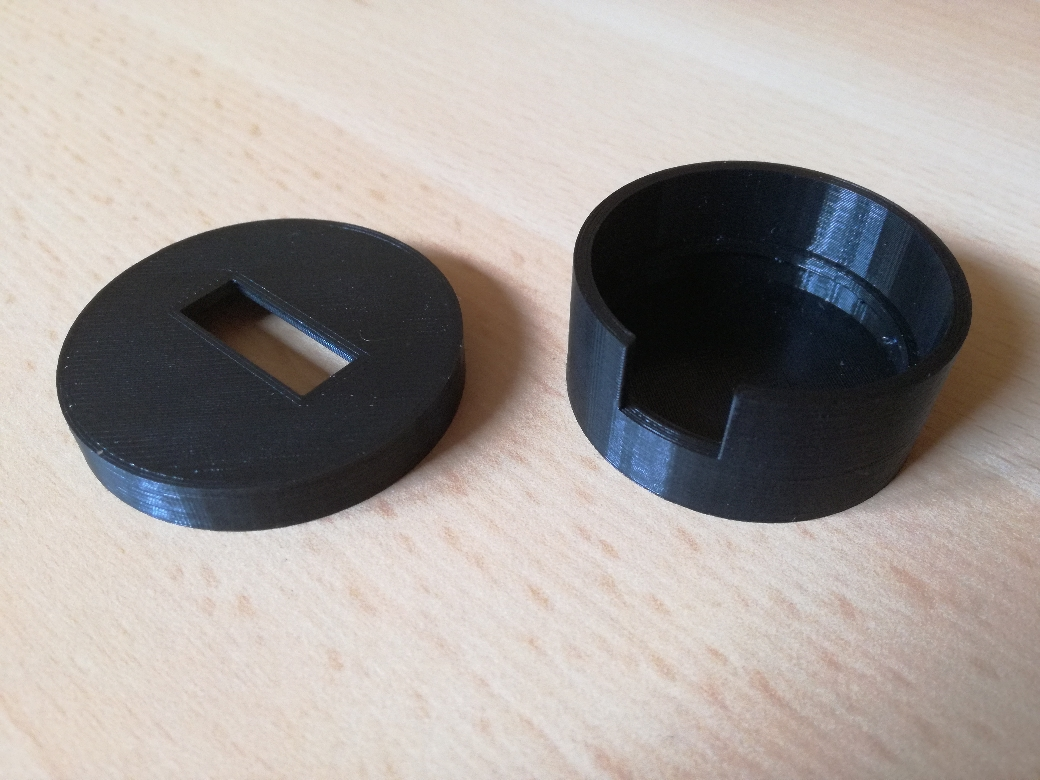
\includegraphics[width=1\textwidth]{Gehauuse_Stimmungslicht.jpg}
 \caption{3D gedrucktes Gehäuse}
 \label{fig:Register}
  \end{center}
\end{figure}


\begin{figure}[!hbpt]
 \begin{center} 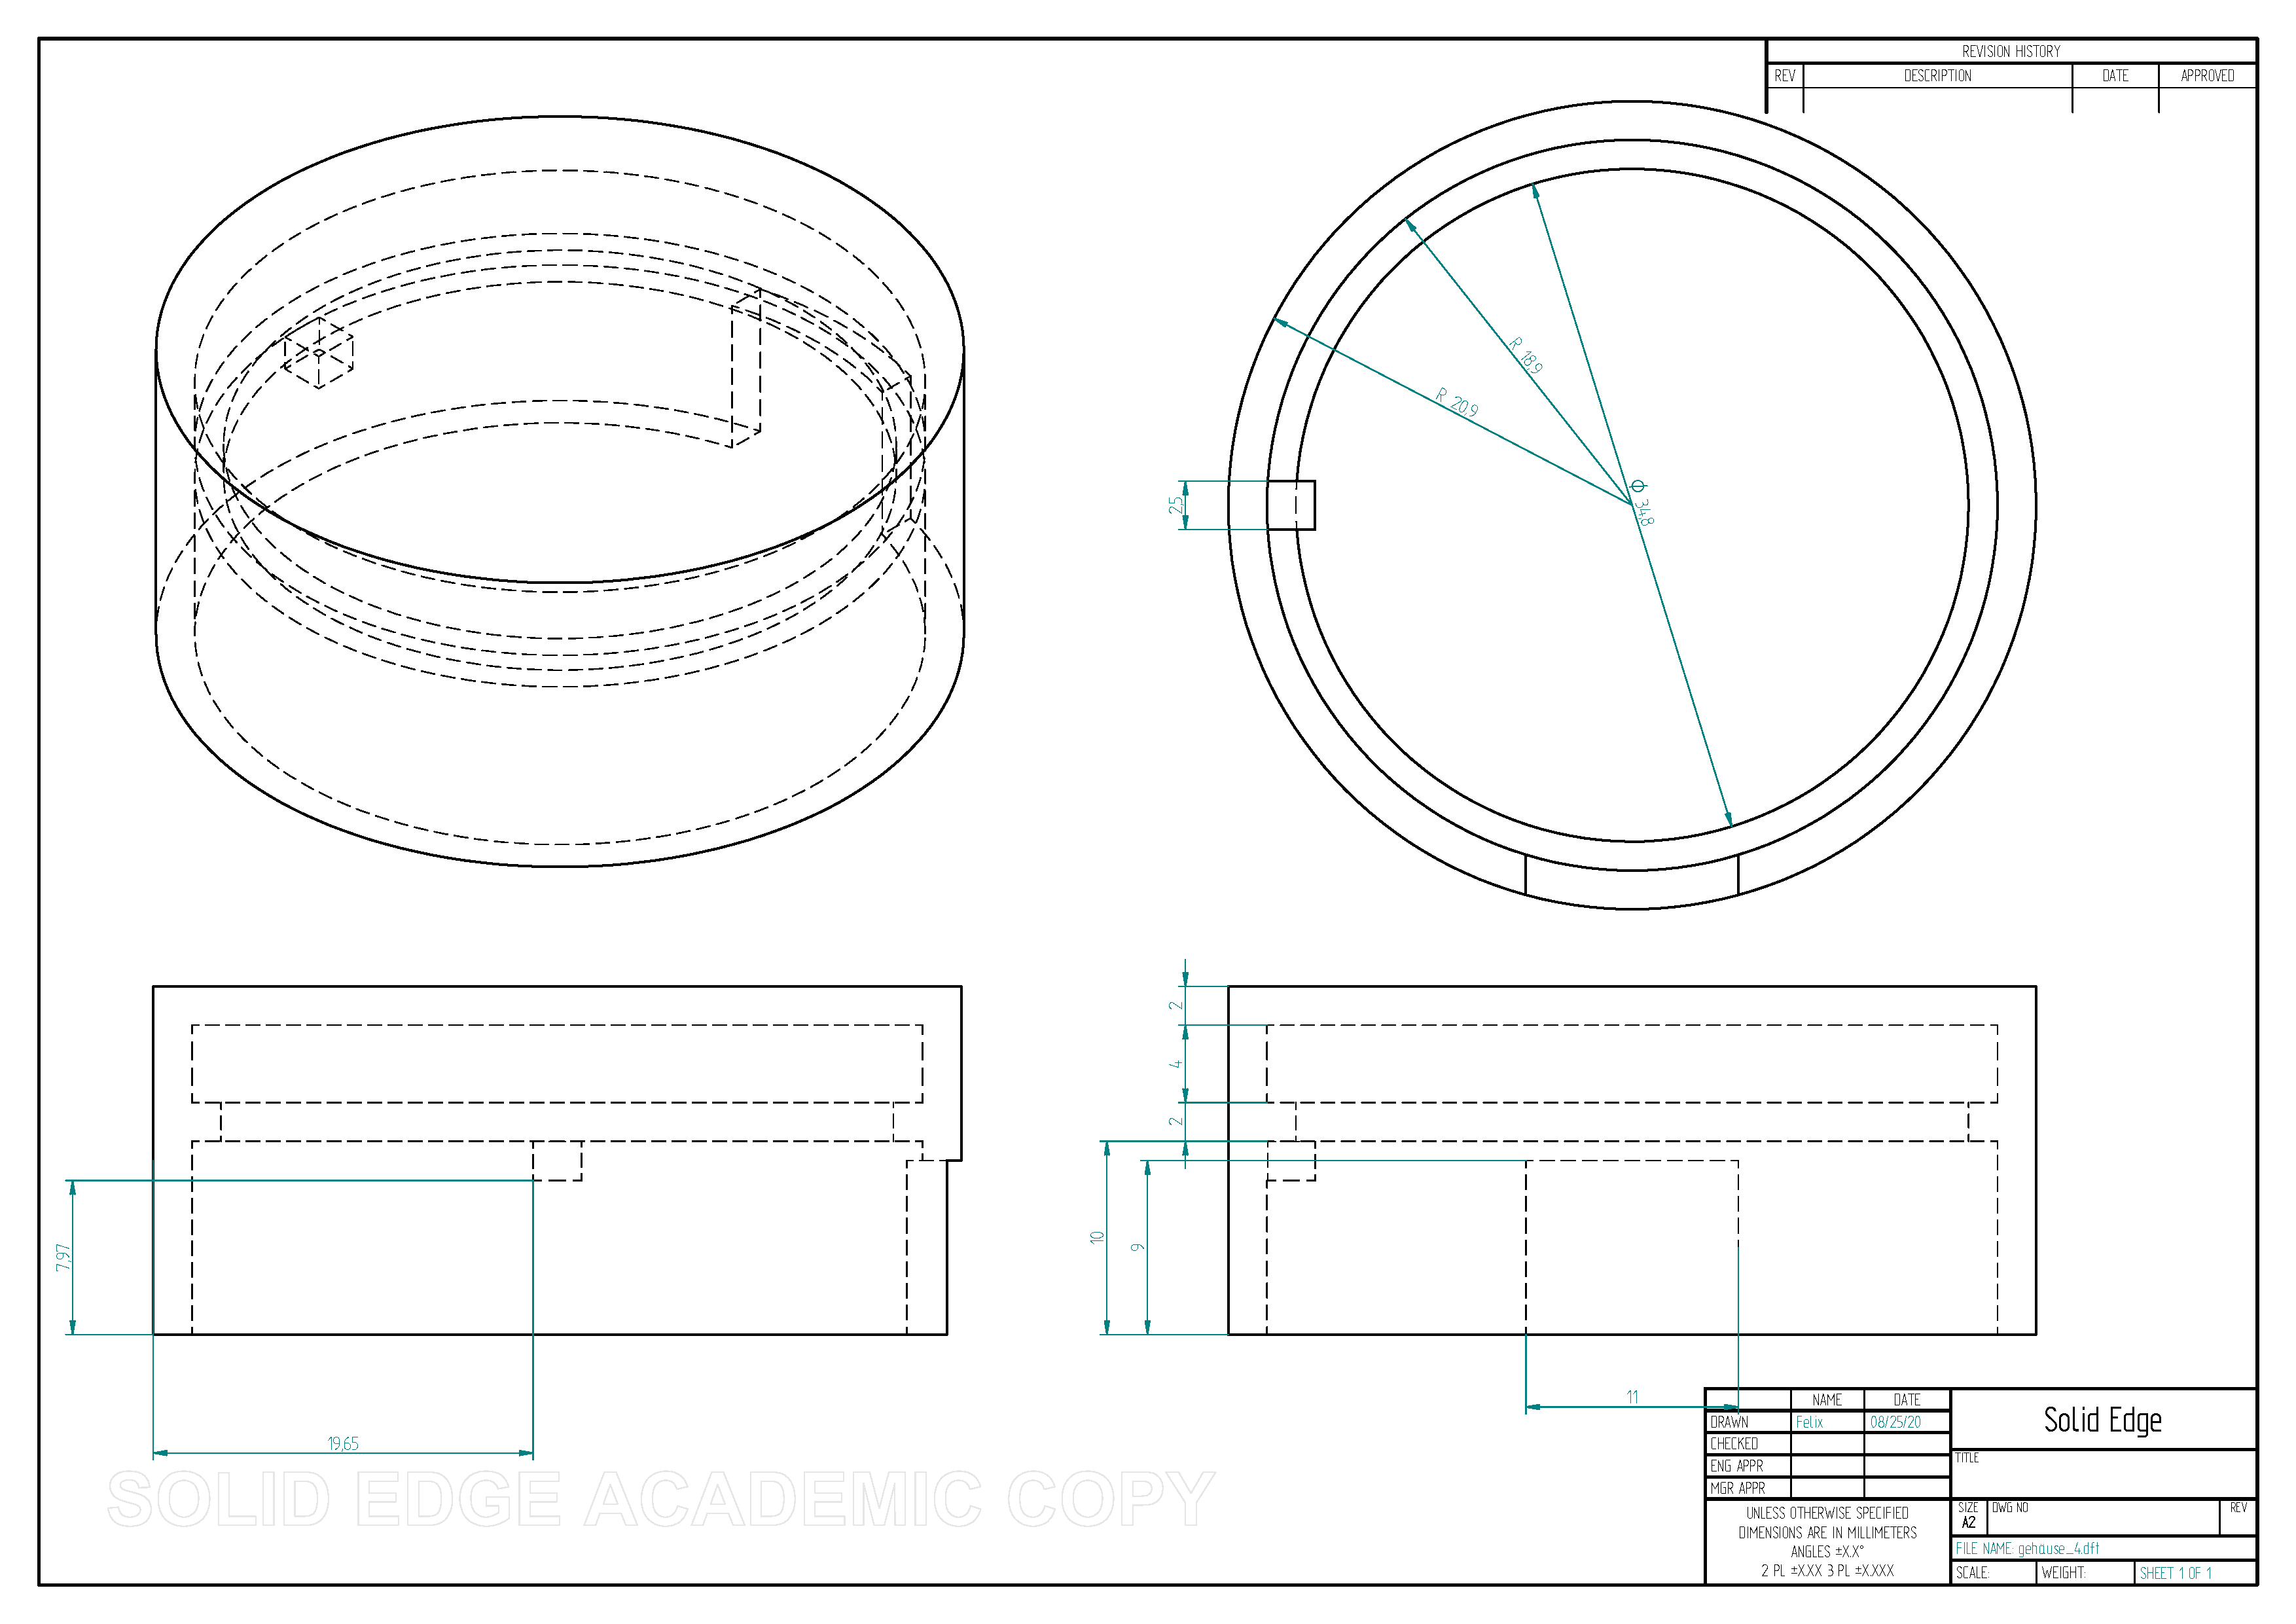
\includegraphics[width=1.4\textwidth,angle=-90]{gehauuse_4.pdf}
 \caption{Grundbehältnis des Gehäuses mit Bemaßungen}
 \label{fig:Register}
  \end{center}
\end{figure}

\begin{figure}[!hbpt]
 \begin{center} \includegraphics[width=1.4\textwidth,angle=-90]{Deckel.pdf}
 \caption{Deckel des Gehäuses mit Bemaßungen}
 \label{fig:Deckel}
  \end{center}
\end{figure}


\section{Fazit}








\cleardoublepage
\begin{appendix}
\listoffigures

\cleardoublepage
\begin{thebibliography}{99}
\bibitem{Nemo} Dr. Nemo: \textit{Submarines through the ages}, Atlantis, 1876.
\end{thebibliography}

\cleardoublepage

\end{appendix}

\end{document}
